\chapter{Fundamentação Teórica}
	\label{ch:fundamentacao}
Neste capítulo serão descritos alguns dos conceitos essenciais para a compreensão do trabalho. Inicialmente é explicado como funciona a organização Baja SAE e as provas as quais os carros são submetidos, além de um breve resumo da história da equipe Velociraptor. Também são descritos alguns detalhes técnicos de quais sensores são/devem ser aplicados no percurso do trabalho além de informações sobre os microcontroladores estudados para servir como base do SCOB vão ser discutidas. Uma análise sobre o protocolo ZigBee é feita e, por último, são discutidos alguns conceitos dos sistemas de tratamento e aquisição de dados.

\section{Baja SAE}
A categoria Baja, organizada pela SAE (\textit{Society of Automotive Engineers}), é uma categoria de \textit{motorsport} feita para estudantes de engenharia aprofundarem seu conhecimento na área com um projeto real, no qual toda a construção do veículo deve ser realizada, bem como sua documentação e busca por patrocinadores para viabilização do projeto. Os carros montados devem, por regulamento, \cite{regulamentobajasae} ser feitos de uma estrutura tubular de aço, fibra de vidro, carbono ou \textit{kevlar} \cite{projetoMiniBaja2006}, com quatro ou mais rodas e motor padrão de 10HP. Também, segundo o regulamento, o carro deve suportar uma pessoa de até um metro e noventa de altura e 113,4 quilogramas de peso. Todo o sistema de suspensão, freio, transmissão e chassi é projetado e executado pela equipe participante.  

As provas realizadas pelos veículos em um torneio, segundo \cite{bajasae} são:
\begin{itemize}
	\item Segurança, testando itens do veículo como gaiola e chassis no quesito de segurança;
	\item Conforto, testando o conforto do piloto ao utilizar o veículo;
	\item Frenagem, testando a capacidade dos freios do veículo;
	\item Suspensão, testando toda a parte de suspensão do veículo em um terreno acidentado;
	\item Capacidade de tração, testando a capacidade do veículo de tracionar puxando uma certa quantidade de peso;
	\item Dirigibilidade, testando o veículo com \textit{slalom}; e
	\item Enduro, uma prova de corrida de longa duração.
\end{itemize}

Além destas provas a equipe também deve realizar uma apresentação com o projeto completo do veículo, contando pontos para o torneio. A equipe que obtiver a maior quantidade de pontos nas provas citadas acima ganha o torneio.

\section{Sensores}
\label{sec:sensores}
Os sensores, junto com atuadores, são os métodos em que circuitos elétricos conseguem se comunicar com o mundo físico realizando algumas tarefas como fazer uma medida de alguma grandeza. Um sensor pode ser definido como um dispositivo que recebe um estimulo e, como resposta, transmite um sinal elétrico \cite{Fraden2016}. Existem diversos tipos de sensores e tipos de variações específicas para cada área de uso, sensores de posição como os potenciômetros, sensores de velocidade angular como tacômetros com rotores dentados, sensores de proximidade com uso de sensores óticos e assim por diante \cite{kilian2001modern}. 

Os sensores presentes em um veículo se dividem em duas categorias \cite{vehicleDataAcquisition2014} - aqueles que são feitos para o conforto do passageiro e aqueles feitos para garantir o devido funcionamento da parte dinâmica do veículo. O primeiro é importante para a lista de opcionais do carro consequentemente agradar ao consumidor comum. O segundo é critico ao engenheiro em alto nível, sem impacto imediato para o publico em geral.

Um bom exemplo de como o sensoriamento pode ajudar no desempenho de uma equipe de automobilismo em tempo real é dado por \citeonline{projetoMiniBaja2006}. Quando superaquecido, o motor fica fora do seu regime ideal de trabalho, causando um maior desgaste dos componentes internos e por consequência uma perda de rendimento, \citeonline{projetoMiniBaja2006} comenta que quando o motor está numa temperatura muito abaixo da ideal, o rendimento também sofre alteração, porque o consumo de combustível aumenta e o torque é menor em relação a um motor ajustado. Para manter o processo dentro de uma faixa desejada, sensores de temperatura do óleo devem ser instalados, com eles é possível manter um histórico da faixa de funcionamento do motor e além de manter o piloto constantemente atualizado da temperatura do motor do seu veículo, o que permite que o piloto tenha mais liberdade em forçar o carro para melhorar o tempo de volta ou dirigir mais cautelosamente, a fim de evitar desgaste excessivo nas peças e melhor consumo de gasolina, fatores que devem ser levados em consideração em uma prova de automobilismo. 

O projeto do veículo \textit{off-road} do grupo Velociraptor já conta atualmente com alguns sensores. A Figura \ref{fig:sensoresBaja} demonstra o esquema do sistema elétrico usado atualmente no veículo. Os espaços em azul são sensores utilizados na competição, os espaços em vermelho são sensores usados para testes de bancada. 


\begin{figure}[!htb]
	\centering
		\caption{Diagrama do sistema elétrico usados atualmente no Baja.}
		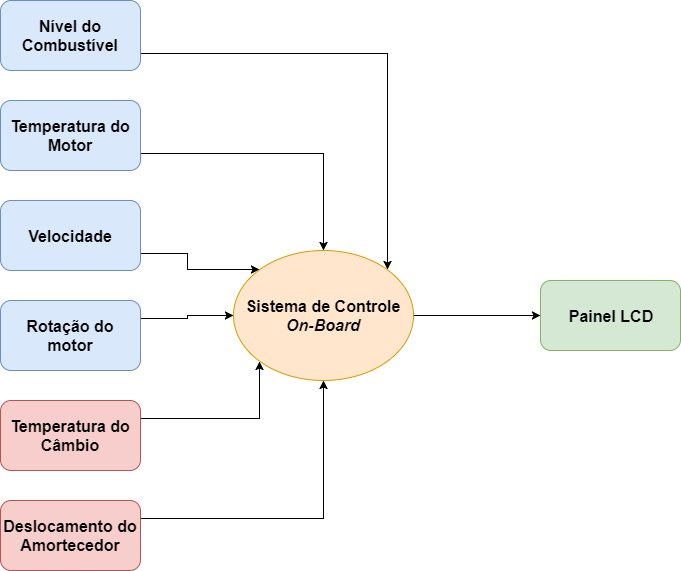
\includegraphics[scale=0.35]{sensoresBaja} 
		\caption*{Fonte: Elaborada pelo autor, 2017.}
		\label{fig:sensoresBaja}
\end{figure} 

\subsection{Temperatura do motor}

O motor deve operar em uma temperatura ideal abaixo de 110$^\circ$C para desempenhar bem o seu papel \cite{Fraden2016}. Se sobreaquecidas, as peças do conjunto começam a operar de forma incorreta e isto pode ocasionar rompimento da junta de vedação da galeria de óleo, diminuição da viscosidade do óleo e em casos de exposição prolongada a sobreaquecimento, travamento do pistão dentro da câmara do motor. Para evitar casos como estes citados acima é importante ter a informação sobre a temperatura do motor, com a informação o piloto pode forçar menos o motor na prova para manter a temperatura estável ou o carro pode ser parado para uma manutenção de emergência.

Para realizar a aquisição desta grandeza é utilizado um sensor termistor de coeficiente negativo de temperatura (conhecido como NTC). Este sensor é facilmente encontrado em lojas de eletrônica, porém o utilizado no projeto Baja Velociraptor é preparado para o ambiente automotivo com um corpo metálico para proteção contra ruídos e melhor posicionamento do sensor. O sensor de temperatura vai acoplado ao cárter do motor, submerso em óleo. O sensor emite um sinal analógico proporcional a temperatura que ele é exposto, a resistência dele diminuí de acordo com o aumento de temperatura e aumenta com temperaturas mais baixas \cite{Fraden2016}. A Figura \ref{fig:sensorTemperaturaautomotivo} é um desenho que apresenta qual a composição deste sensor de caráter automotivo.   

\begin{figure}[!htb]
	\centering
		\caption{Variante do termistor para aplicação automotiva.}
		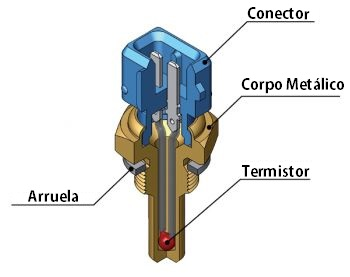
\includegraphics[scale=0.6]{sensorTemperaturaautomotivo} 
		\caption*{Fonte:\cite{sensortempauto} modificado pelo autor.}
		\label{fig:sensorTemperaturaautomotivo}
\end{figure} 



\subsection{Frequência de rotação do motor}

A revolução/rotação por minuto (RPM) é uma grandeza que indica quantas rotações por minuto um certo objeto realiza, sendo em torno de si mesmo ou em torno de um outro objeto \cite{Dias2010}. No contexto do automobilismo, a RPM é a quantidade de vezes em que um motor realiza um giro completo, movendo o virabrequim que está conectado a uma transmissão. Esta transmissão por sua vez está conectada a um eixo e consequentemente o eixo está conectado a roda. Esta é uma ideia básica de como funciona o sistema de conversão de um fenômeno químico (combustão do motor) em força física e o que a RPM trata neste meio.

Para fazer aquisição desta grandeza, uma das técnicas possíveis para retirada dessa grandeza envolve a vela automotiva\cite{projetoMiniBaja2006}. A vela está presente em todos os carros movidos a motores de combustão a gasolina, sua função é causar a centelha que começa o processo de explosão do combustível misturado com ar na câmara interna do motor.       

A vela produz uma centelha a cada ciclo de explosão da gasolina e esta centelha é produzida a partir de uma descarga de energia com tensão de 12KV\cite{projetoMiniBaja2006}. A carga de energia é capturada por uma bobina em volta do fio elétrico da vela e conectada a uma entrada digital do microprocessador. Quando ocorrer a centelha é executada uma interrupção no programa do microprocessador e incrementado um valor em uma variável reservada para a RPM. Esta variável ainda deve ser tratada antes de ser passada para o painel pois a centelha da vela é ativada uma vez a cada ciclo do motor, porém dentro de um ciclo completo (admissão, compressão, explosão e exaustão) é realizado dois giros do virabrequim, ou seja, duas RPM. Depois de ter o valor multiplicado por dois, o valor é mostrado no painel. 

\subsection{Velocidade do veículo}

A velocidade do veículo é a grandeza que indica a quão rápido um veículo se move de um ponto A para um ponto B. Para aquisição desta grandeza é utilizado um sensor MTE 73020. Este sensor vai acoplado perto do eixo do veículo e captura a rotação do mesmo graças ao efeito Hall, esta rotação é transformada em uma onda quadrada \cite{MTEsensorVelocidade} e que deve ser tratada de acordo com a sua aplicação. Este tipo de sensor é utilizado em carros da montadora General Motors.  

No Baja Velociraptor o sensor está acoplado ao eixo traseiro, próximo ao motor, e captura a rotação do freio traseiro que está conectado ao eixo. A Figura \ref{fig:sensorVelocidadeEx} apresenta como este sensor está acoplado em direção ao disco do freio. A todo momento que um dente do freio passa próximo ao sensor o mesmo emite um sinal que está conectado a entrada digital do microprocessador no SCOB. A frequência recebida pelo SCOB é tratada, levando em consideração o tamanho da roda e número de dentes no freio, resultando na fórmula matemática:

	$$V = \frac{S_{vel}}{N_{freio}} \times 2 \pi r  \times \frac{3.6km}{h},$$  

Sendo $V$ é a velocidade final mostrada no painel, $S_{vel}$ é o número de vezes que o sensor produziu uma sinal quadrada, $N_{freio}$ é a quantidade de dentes presente no freio customizado do Baja Velociraptor, $2 \pi r$ é fórmula do comprimento da circunferência e $\frac{3.6km}{h}$ transforma o resultado de metros por segundo para quilômetros por hora. Esta fórmula já era utilizada no sistema de aquisição de dados desenvolvido pelos membros do sub-sistema da eletrônica embarcada.

\begin{figure}[!htb]
	\centering
		\caption{Sensor de velocidade conectado próximo ao freio traseiro.}
		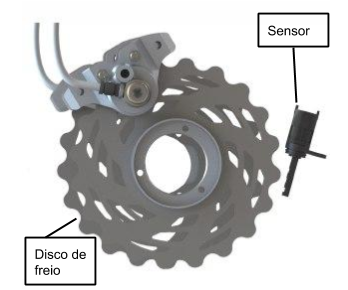
\includegraphics[scale=0.5]{sensorVelocidadeEx} 
		\caption*{Fonte: UDESC Baja Velociraptor (2017).}
		\label{fig:sensorVelocidadeEx}
\end{figure} 


\subsection{Nível do combustível}
\label{subsec:combustivel}

O combustível é utilizado para causar a explosão controlada dentro do motor de combustão. Medir a quantidade ainda disponível no tanque de gasolina dele é essencial para que possam ser tomadas decisões como manter o veículo na pista ou chamar o veículo para os boxes. A técnica mais comum utilizada para medir esta grandeza é a boia, como pode ser visto em alguns trabalhos analisados (\cite{Nunes2016} e \cite{projetoMiniBaja2006}) mas esta técnica não pode mais ser aplicada nas competições devido a novas regras de competição que não permitem uso de fios dentro de motores ou tanques de combustível \cite{regulamentobajasae}. 

Para se adequar a estes novos regulamentos, foi utilizada uma nova técnica de medida da grandeza. Esta técnica consiste em utilizar uma boia dentro do tanque de gasolina com um imã e 5 sensores de efeito Hall US1881 fixados na parte externa do tanque. Os sensores de efeito Hall tem seu valor de saída alterado quando a boia presente dentro do tanque passa por eles, desta forma é possível medir a quantidade de gasolina dentro do tanque sem que exista a necessidade de fios na parte interna do mesmo. A sinal de saída desses sensores é digital, mas para melhor manutenção dos chicotes elétricos este sinal é convertido para um sinal analógico, no qual a frequência recebida pelo microcontrolador é proporcional a quantidade de gasolina presente no tanque. A Figura \ref{fig:sensorTanque} mostra como é montado o \textit{shield} com os sensores de efeito Hall enfileirados.  

\begin{figure}[!htb]
	\centering
		\caption{\textit{Shield} criado para sensores de efeito Hall US1881.}
		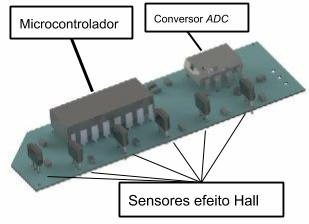
\includegraphics[scale=0.7]{sensorTanque} 
		\caption*{Fonte: UDESC Baja Velociraptor (2017).}
		\label{fig:sensorTanque}
\end{figure} 


\subsection{Temperatura do câmbio CVT}

O motor a combustão de um veículo gera torque e potência, porém esta entrega é linear e pode ser ineficaz dependendo do terreno em que o veículo se encontra. Para contornar esta situação e ter sempre o torque desejado, é adicionada uma transmissão ao veículo. A transmissão converte a saída de torque e potência com o objetivo de manter o motor o mais próximo possível da hipérbole de tração ideal \cite{Naunheimer2011}. 

O tipo de transmissão escolhida para o Baja Velociraptor foi uma caixa de câmbio CVT (\textit{Continuosly Variable Transmission}). Para a equipe, a informação da temperatura da transmissão é importante para o projeto do veículo pois o câmbio CVT possui componentes sensíveis como a correia utilizada no sistema. 

Para obter essas informações do câmbio foi utilizado um sensor MLX90614 (Figura \ref{fig:sensorCvt}\subref{fig:sensorCvtimg}). Este sensor, da categoria termopilha, opera utilizando o mesmo princípio de um sensor termopar. Um termopar simples é um dispositivo de baixa sensibilidade que responde a mudanças da casa de 1$^\circ$C com uma mudança de dezenas de $\mu V$, um sensor de termopilha é uma cadeia de termopares conectados, tipicamente 50 a 100 junções, para obter um sinal de 50 a 100 vezes mais forte. O sensor opera com uma membrana com uma capacidade térmica baixa devido a seu tamanho, e esta membrana varia de temperatura de acordo com a radiação térmica para que desta forma a temperatura seja calculada gerando uma tensão correspondente \cite{Fraden2016}. A Figura \ref{fig:sensorCvt}\subref{fig:sensorCvtfunc} exemplifica o que é explicado no paragrafo anterior, mostrando o processo de atuação do sensor. A saída deste sensor é dada em valores analógicos porém vai conectada a uma entrada digital do microcontrolador devido ao uso do protocolo I$^2$C.       

\begin{figure}[!htb]
	\center
	\caption{Sensor MLX90614 e seu funcionamento.}
	\subfigure[Fonte:Google Imagens][Sensor MLX90614. Fonte:\cite{tempcvt}]{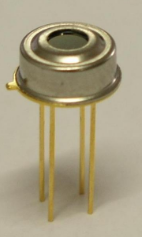
\includegraphics[width=3cm]{sensorCvt}\label{fig:sensorCvtimg}}
	\qquad
	\subfigure[Fonte:\cite{Fraden2016}][Exemplo do funcionamento. Fonte:\cite{Fraden2016}]{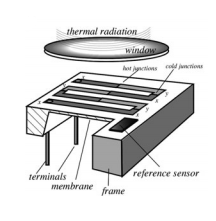
\includegraphics[width=5cm]{sensorCvtfunc}\label{fig:sensorCvtfunc}}
	\label{fig:sensorCvt}
\end{figure}

\subsection{Célula de carga}
A célula de carga é um sensor que transforma grandeza física em sinal elétrico. Ele funciona a partir do princípio da variação da resistência ôhmica de um extensômetro quando este é submetido a alguma força \cite{Fraden2016}. Esta deformação então é transformada em uma saída de tensão que é capturada pela porta analógica do microcontrolador.

Este sensor foi utilizado para verificar a ação de forças sobre o \textit{link} da suspensão, uma das peças responsáveis por manter os pneus na cambagem correta. O modelo utilizado foi o Z-20 devido a sua disponibilidade no mercado e também a sua capacidade de carga de até uma tonelada.   

\subsection{Deslocamento do amortecedor}

O amortecedor, que está contido no conjunto da suspensão, tem o papel de controlar o carro de forma a manter as rodas do veículo em constante contato com o solo, trazendo melhor desempenho para o mesmo. Este sensor de deslocamento de amortecedor é utilizado em bancada para testes e para realização da aquisição da grandeza, neste caso a distância de deslocamento, foi criado um instrumento semelhante a um amortecedor em cano PVC e este instrumento fica acoplado ao lado do amortecedor. Quando o amortecedor sofre tensão o esforço também é transmitido para o instrumento e nele é realizada a aquisição da grandeza. Estes dados adquiridos ajudam na tomada de decisão da configuração da suspensão, escolhendo entre uma suspensão mais rígida ou mais suave dependendo do terreno, calibragem dos pneus, etc.

É utilizado um sensor GP2Y0A21YK0F da SHARP para fazer a aquisição do deslocamento do amortecedor. Este sensor vai acoplado em uma das pontas do cano, apontado para a outra. A distância efetiva de operação do sensor é de 10cm - 80cm \cite{SHARP} o que é suficiente para o cenário. O sinal resultante da aquisição é analógico e proporcional a distância do sensor em relação ao objeto em que ele está apontado. 

\section{Microcontroladores}
\label{sec:microcontroladores}

Os microcontroladores são os dispositivos de maior importância dentro de um sistema embarcado, sendo considerados o coração de um projeto que envolva soluções remotas \cite{aSurveyTo2010}. O microcontrolador possui várias funções integradas dentro de um único \textit{chip} e com baixo consumo de energia. Dentro dele é possível encontrar uma unidade de processamento, uma quantidade fixa de memória RAM, memória ROM, pinagem para operações gerais de entrada e saída, entradas/saídas para protocolos seriais como \textit{I$^2$C} além de um \textit{timer} \cite{mazidi2008pic}. A Figura \ref{fig:arquiteturaAtmega} é um exemplo a arquitetura de um microcontrolador usado em diversas placas de desenvolvimento, o ATmega328/ATmega328p. Ele utiliza arquitetura Harvard, ou seja, o acesso a memória de dados é separado da memória de programa.        


\begin{figure}[!htb]
	\centering
		\caption{Diagrama de blocos do microcontrolador ATmega328/ATmega328p.}
		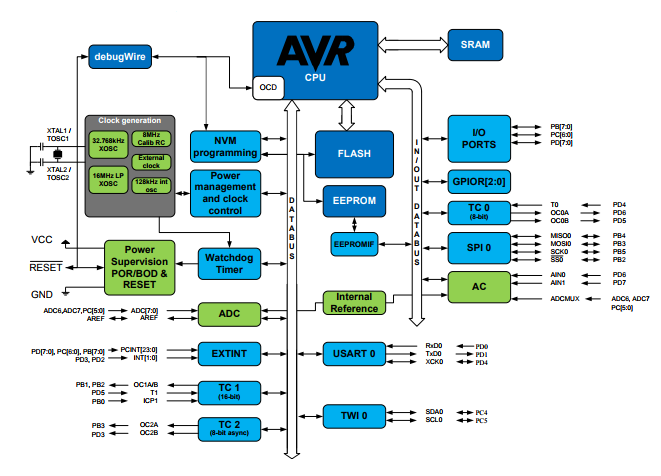
\includegraphics[scale=0.7]{arquiteturaAtmega} 
		\caption*{Fonte: \cite{atmel}.}
		\label{fig:arquiteturaAtmega}
\end{figure} 

Em \citeonline{aSurveyTo2010} e em \citeonline{mazidi2008pic} são citados alguns fatores que são levados em conta na escolha do microcontrolador, porém tais critérios podem ser revistos e redimensionados para a aplicação no Baja Velociraptor. Os critérios de maior relevância então são:

\begin{itemize}
	\item Baixo consumo de energia para melhor dimensionamento da bateria;
	\item Quantidade de RAM e ROM suficiente para a rotina desejada a fim de guardar variáveis importantes durante o tempo de execução do código no microcontrolador;
	\item Quantidade suficiente de entradas/saídas para periféricos; 
	\item Programável em C, devido ao conhecimento da equipe na linguagem; e
	\item Custo, com valores entre R\$50 e R\$150.
\end{itemize}   

A equipe Velociraptor atualmente já trabalha com um microcontrolador da Atmel, o ATmega328 em uma placa de desenvolvimento Arduino Nano V3. Este microcontrolador supre todos os critérios citados acima para o cenário atual, com os sensores citados na subseção \ref{sec:sensores}, porém com a criação de um novo \textit{software} para tratamento de dados e em conjunto com os objetivos futuros da equipe de atualizações nas tecnologia utilizadas, o uso deste microcontrolador deve ser revisado para ser mantido ou descartado. Outro fator discutido com a equipe é o uso de microcontroladores que são suportados por placas de desenvolvimento, revisadas na seção \ref{sec:placasdedesenvolvimento}. As placas de desenvolvimento facilitam a criação do SCOB, e servem para o escopo deste projeto já que são placas desenvolvidas para um ambiente de prototipagem. 

O Quadro \ref{tab:microcontroladores} faz uma comparação entre microcontroladores encontrados em placas de desenvolvimento no mercado das marcas Intel\footnote{\href{https://www.intel.com/content/dam/www/public/us/en/documents/datasheets/quark-c1000-datasheet.pdf}{Quark SE Microcontroller C1000 Datasheet}}, Atmel\footnote{\href{http://www.atmel.com/Images/Atmel-7766-8-bit-AVR-ATmega16U4-32U4_Datasheet.pdf}{ATmega16U4/ATmega32U4 Datasheet}}\footnote{\href{http://www.atmel.com/Images/Atmel-42735-8-bit-AVR-Microcontroller-ATmega328-328P_Datasheet.pdf}{ATmega328/P Datasheet}}\footnote{\href{http://www.atmel.com/Images/Atmel-2549-8-bit-AVR-Microcontroller-ATmega640-1280-1281-2560-2561_datasheet.pdf}{Atmel ATmega640/V-1280/V-1281/V-2561/V Datasheet}}\footnote{\href{http://www.atmel.com/Images/Atmel-11057-32-bit-Cortex-M3-Microcontroller-SAM3X-SAM3A_Datasheet.pdf}{SAM3X / SAM3A Series Datasheet}} e NXP\footnote{\href{https://www.nxp.com/docs/en/data-sheet/KL25P80M48SF0.pdf}{NXP Kinetis KL25 Sub-Family Datasheet}} . 
O microcontrolador com maior poder de processamento é o AT91SAM3X8E com velocidade de \textit{clock} 5.25 vezes maior que o microcontrolador mais lento e 48 vezes mais memória. O microcontrolador da Intel possui uma boa quantidade de memoria RAM, porém sua pinagem é menor que do ATmega328, o microcontrolador de menor desempenho da família Atmel visto neste comparativo. 
\begin{table}[!htb]
	\centering
	\caption{Comparação de microcontroladores.}
	\label{tab:microcontroladores}
	\begin{tabular}{|l|l|l|l|l|l|}
		\hline
		\rowcolor[HTML]{9B9B9B} 
		\textbf{Modelo}  & \textbf{Fabricante} & \textbf{Clock} & \textbf{I/O Digital} & \textbf{I/O Analógica} & \textbf{RAM} \\ \hline
		AT91SAM3X8E    & Atmel               & 84 MHz         & 54                   & 14                     & 96 KB SRAM   \\ \hline
		ATmega2560     & Atmel               & 16 MHz          & 54                   & 16                     & 8 KB SRAM    \\ \hline
		ATmega328     & Atmel               & 16 MHz         & 14                   & 8                      & 2 KB SRAM    \\ \hline
		ATmega32u4     & Atmel               & 16 MHz          & 20                   & 12                     & 2.5 KB SRAM  \\ \hline
		MKL25Z128VLK4  & NXP                 & 48 MHz          & 60                   & 6                      & 16 KB SRAM   \\ \hline
		Quark SE C1000 & Intel               & 32 MHz         & 14                   & 6                      & 80 KB SRAM   \\ \hline
		\end{tabular}
	\caption*{Fonte: Autor.}
\end{table}

\subsection{Placas de desenvolvimento} 
\label{sec:placasdedesenvolvimento}

O mercado atual de sistemas embarcados oferece uma opção para melhor produtividade e facilidade de desenvolvimento, a custo da especificidade envolvida nos projetos. As placas de desenvolvimento são componentes criados para suportar um ambiente com uma unidade de processamento, geralmente um microcontrolador, um cristal gerador de \textit{clock} e uma entrada para interfaceamento com o computador (USB ou mini-USB), outros periféricos também podem ser encontrados de fábrica dependendo do modelo, como acelerômetros e giroscópios. 

Estas placas de desenvolvimento possuem diversos microcontroladores, fabricantes, tamanhos, poder de processamento, poder de armazenamento e assim por diante. O Quadro \ref{tab:placasdedesenvolvimento} traz uma comparação entre várias placas de desenvolvimento que utilizam microcontroladores vistos no Quadro \ref{tab:microcontroladores}. A dimensão é dada em milímetro, todas as placas tiveram seus preços verificados no mês de novembro do ano 2017 em um \textit{e-commerce} de componente eletrônicos\cite{filipeflop}. A dimensão de altura das placas Arduino são estimativas, visto que oficialmente estes números não são divulgados. 

\begin{table}[!htb]
	\centering
	\caption{Comparação entre placas de desenvolvimento}
	\label{tab:placasdedesenvolvimento}
	\begin{tabular}{|l|l|l|l|l|}
	\hline
	\rowcolor[HTML]{9B9B9B} 
	\textbf{Modelo}      & \textbf{Fabricante} & \textbf{Microcontrolador} & \textbf{Dimensões (mm)} & \textbf{Preço} \\ \hline
	FRDM-KL25Z		   & NXP                 & MKL25Z128VLK4             & 80 x 53 x 6        & R\$169,90      \\ \hline
	Genuino 101        & Intel               & Quark SE                  & 70 x 55 x 20       & R\$229,90      \\ \hline
	Uno R3             & Arduino             & ATmega328                 & 68.6 x 53.4 x 25   & R\$44,90       \\ \hline
	Nano V3            & Arduino             & ATmega328                 & 45 x 18 x 7.6      & R\$49,90       \\ \hline
	Mega 2560 R3       & Arduino             & ATmega2560                & 102 × 54 x 25      & R\$74,90       \\ \hline
	Due                & Arduino             & AT91SAM3X8E               & 101.52 x 53.3 x 25 & R\$139,90      \\ \hline
	Leonardo R3        & Arduino             & ATmega32u4                & 68.6 x 53.3 x 25   & R\$59,90       \\ \hline
	\end{tabular}
	\caption*{Fonte: Autor.}
\end{table}

É possível tirar algumas análises deste quadro, por exemplo, o Arduino Nano V3 possui o mesmo poder de processamento de um Arduino Uno R3 porém utiliza uma área aproximadamente 4.5 vezes menor do que o mesmo, custando uma pequena margem a mais. Levando em conta o cenário do projeto, as \textbf{dimensões} de uma placa de desenvolvimento é um fator que também deve ser levado em conta na tomada de decisão, o que não se aplicava a microcontroladores pois estes possuem um tamanho pequeno em comparação com placas de desenvolvimento que possuem alguns componentes extras já citados no início da seção. Algumas placas como Genuino 101, Due e FRDM-KL25Z possuem um preço que varia acima da casa dos R\$100. Isto pode ser justificado com desempenho superior em relação as demais placas e alguns periféricos extras já inclusos nestas placas, como acelerômetro em ambas FRDM-KL25Z e Genuino 101. Placas com dimensões como o modelo Mega 2560 R3 não são a melhor opção para ser utilizadas no veículo para uso durante a prova visto a impossibilidade de criar um \textit{shield} para proteção da mesma e acoplamento no painel dianteiro do veículo. A Figura \ref{fig:paineldianteiro} mostra como está estruturado o painel atualmente com um Arduino Nano V3. Este mesmo painel é feito em alumínio protege o SCOB de vários fatores externos como lama e água, a figura também mostra as fiações elétricas que chegam no painel e algumas partes mecânicas como fluído de freios e pedais de aceleração/frenagem. Uma mudança de tamanho requisitaria uma revisão do projeto de eletrônica do veículo.

\begin{figure}[!htb]
	\centering
		\caption{Foto do painel dianteiro atual do Baja Velociraptor.}
		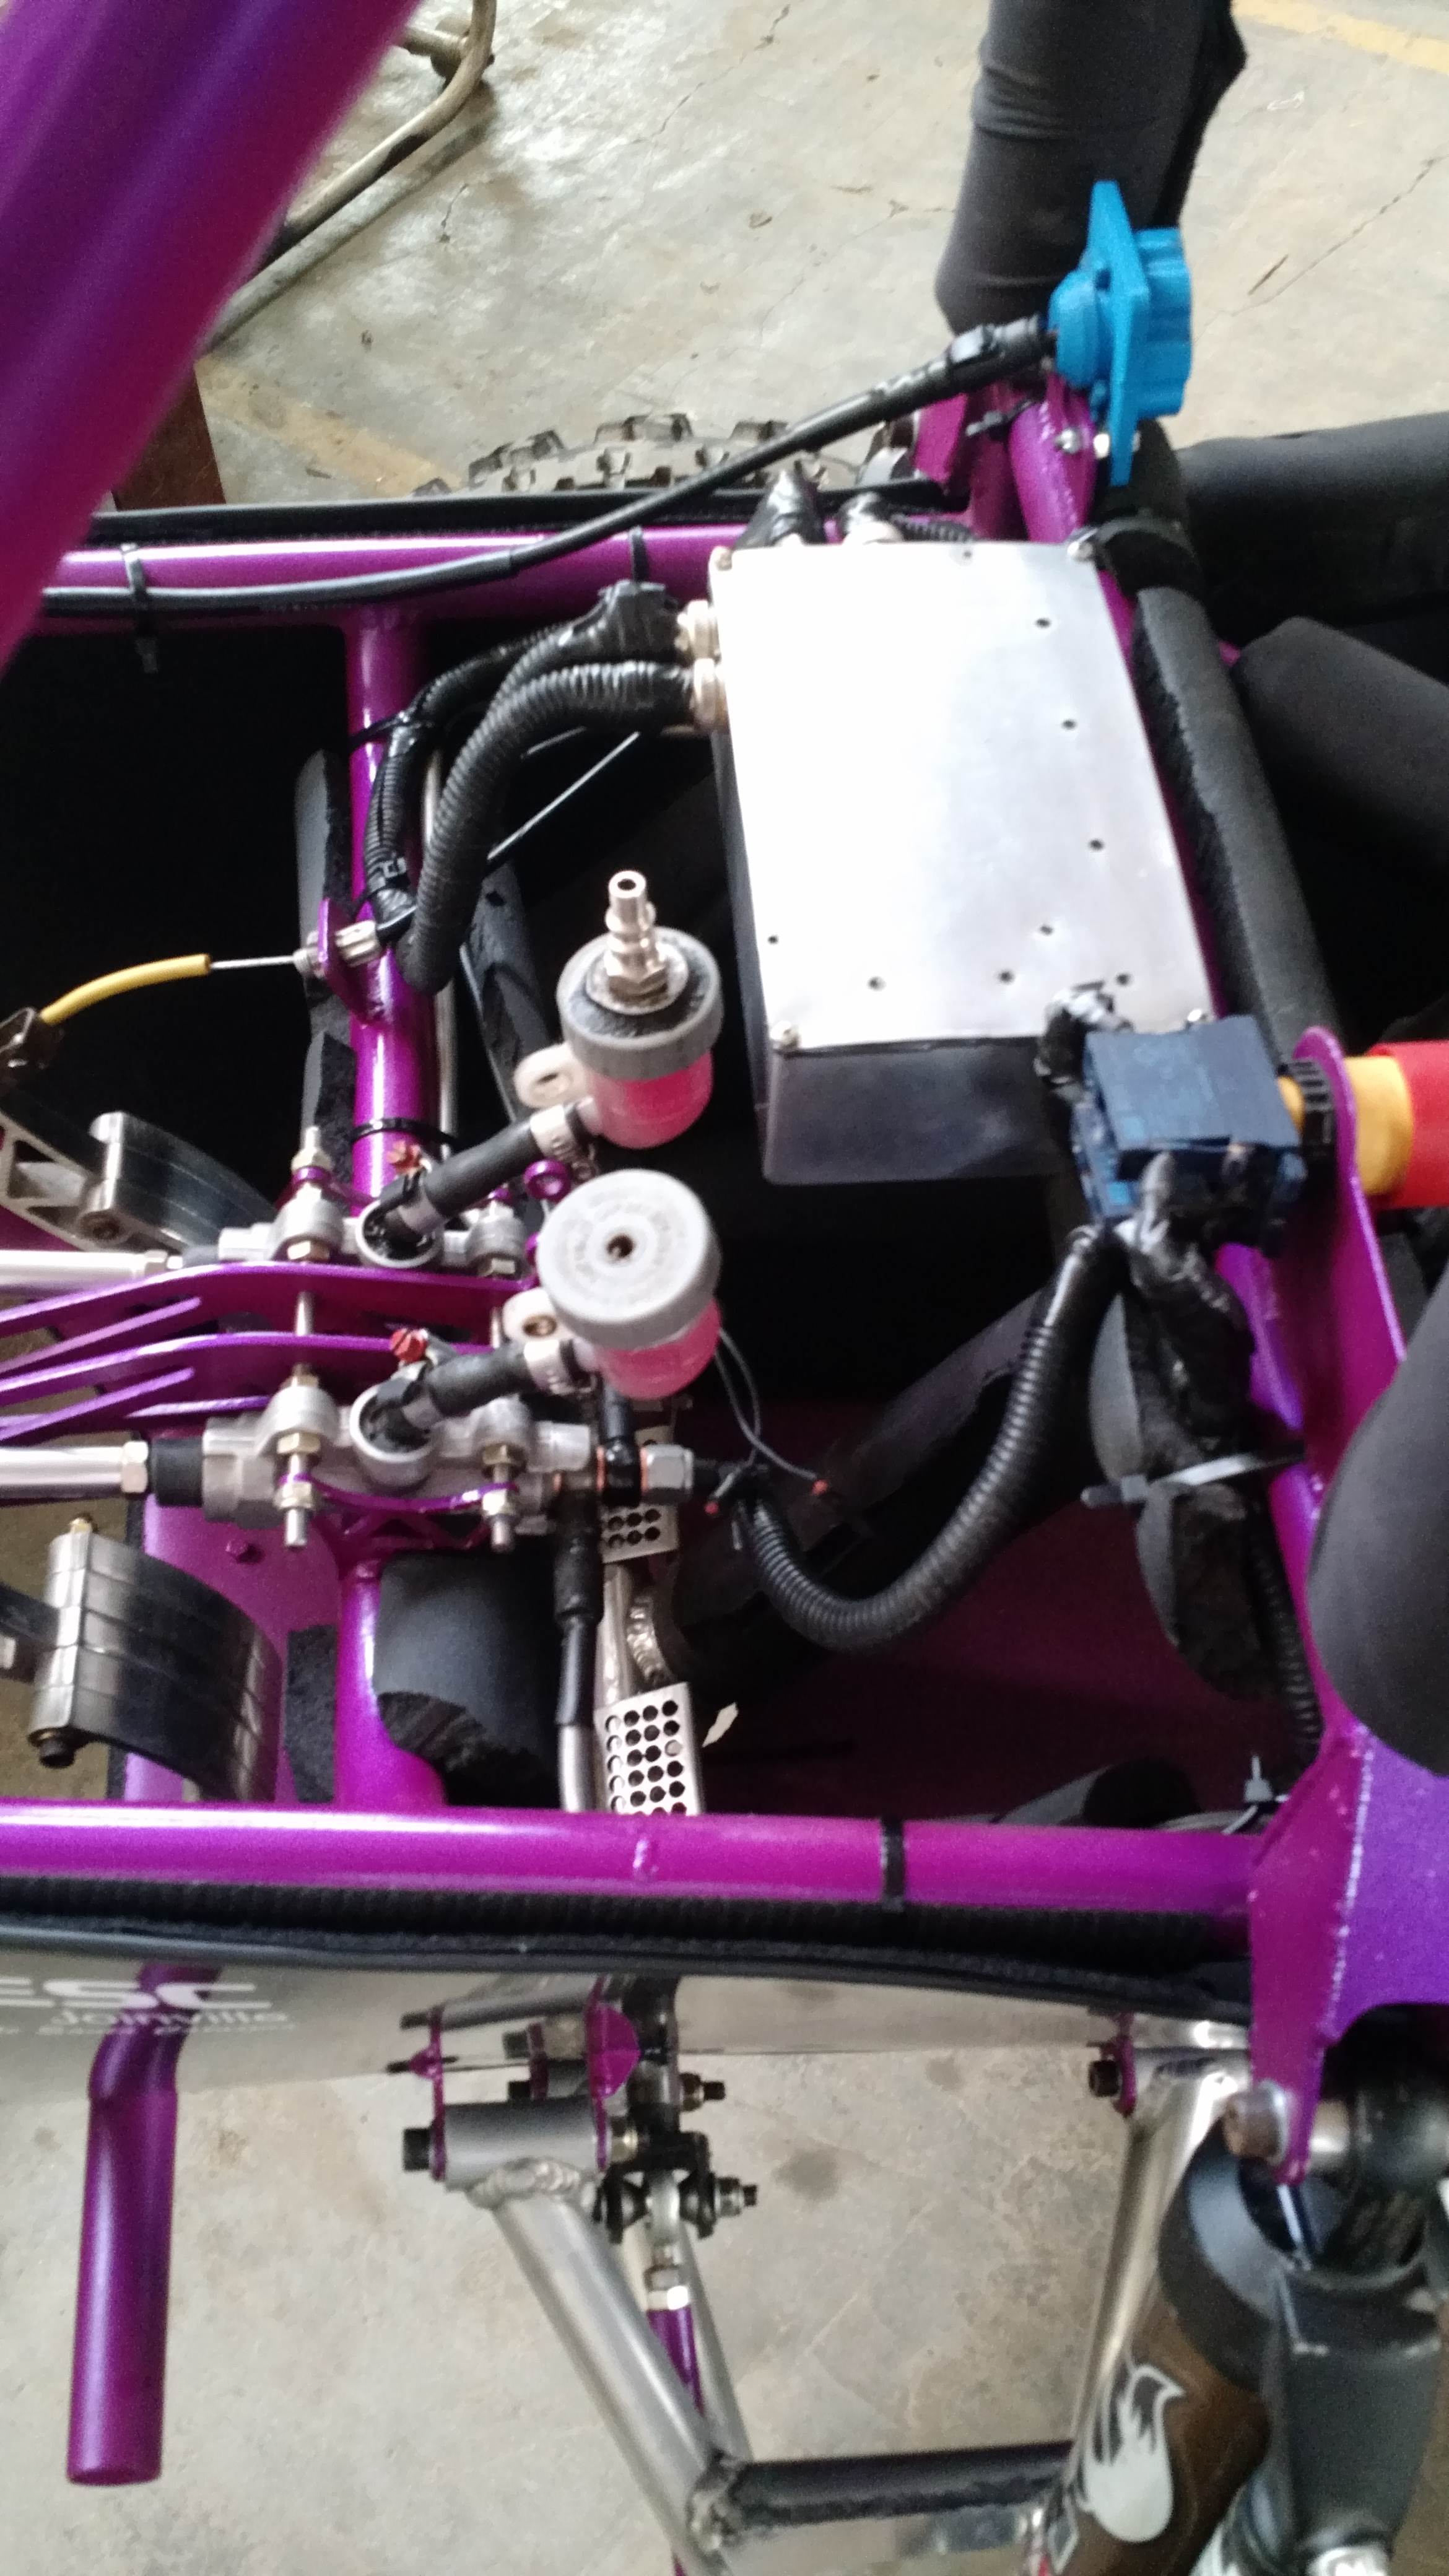
\includegraphics[scale=0.05]{paineldianteiro} 
		\caption*{Fonte: Autor.}
		\label{fig:paineldianteiro}
\end{figure} 
     

Todavia, além das placas de desenvolvimento citadas, \citeonline{designAndImplementation2015} traz uma solução de aquisição de dados para veículos (mais informações do trabalho no Capítulo \ref{ch:trabalhos}) com o uso de placas de melhor desempenho, com maior número de periféricos porém ainda em uma escala reduzida. Este tipo de placa é comumente chamado de \textit{Single Board Computer} por serem capazes de executar um sistema operacional completo, e não apenas um programa como nas placas analisadas no Quadro \ref{tab:placasdedesenvolvimento}. O Quadro \ref{tab:singleboard} tem a comparação de algumas destas \textit{Single Board Computer} na qual as dimensões são dadas em milímetros, todas as placas tiveram seus preços verificados no mês de novembro do ano 2017 em um \textit{e-commerce} de componente eletrônicos\cite{filipeflop}.

\begin{table}[!htb]
	\centering
	\caption{Comparação entre \textit{Single Board Computer}}
	\label{tab:singleboard}
	\resizebox{\textwidth}{!}{\begin{tabular}{|l|l|l|l|l|l|l|l|l|}
		\hline
		\rowcolor[HTML]{9B9B9B} 
		\textbf{Modelo} & \textbf{Fabricante} & \textbf{Processador}     & \textbf{Clock} & \textbf{I/O Digital} & \textbf{I/O Analógica} & \textbf{RAM}  & \textbf{Dimensões} & \textbf{Preço} \\ \hline
		3 Model B     & Raspberry Pi        & BCM2837         & 1200 MHz       & 40                   & N/A                    & 1 GB LPDDR2   & 85 x 56 x 17       & R\$299,90      \\ \hline
		Zero W        & Raspberry Pi        & BCM2835         & 1000 MHz       & 40                   & N/A                    & 512 MB LPDDR2 & 65 x 30 x 5        & R\$79,90       \\ \hline
		Green         & BeagleBone          & AM3358 & 1000 MHz       & 65                   & 7                      & 512 MB DDR3   & 86 x 53 x 19       & R\$329,90      \\ \hline
		Black Rev.C   & BeagleBone          & AM3358 & 1000 MHz       & 65                   & 7                      & 512 MB DDR3   & 86 x 53 x 19       & R\$399,90      \\ \hline
	\end{tabular}}
	\caption*{Fonte: Autor.}
\end{table}

Os modelos 3 Model B, Green e Black Rev.C possuem um preço acima da faixa de R\$250 e dificilmente serão escolhidos para o projeto, porém de todas as \textit{Single Board Computer} comparadas, o modelo Zero W tem a proposta mais atraente. Com memória RAM de 512 MB, velocidade de \textit{clock} de 1.000 MHz, dimensões 65 x 30 x 5 milímetros e preço R\$79,90 esta \textit{Single Board Computer} possui poder de processamento e memória acima dos modelos vistos no Quadro \ref{tab:placasdedesenvolvimento} por um preço abaixo da casa de R\$100. A utilização dessas placas ainda traz vantagens como a possibilidade de rodar um sistema operacional dentro do veículo, o que pode ser explorado para melhor processamento de dados dentro do SCOB, utilização de linguagens interpretadas e utilização de sistemas gerenciadores de bancos de dados para adição de uma camada extra de confiabilidade nos dados entregues pelo sistema. A desvantagem da utilização deste sistema é o custo, que aumenta uma margem pequena (cerca de 1.6 vezes o valor atual da placa de desenvolvimento), o aumento da complexidade do sistema com a adição de um sistema operacional dentro do veículo, o aumento das dimensões da placa de desenvolvimento (de 45 x 18 x 7,6 para 65 x 30 x 5) e a falta de entradas analógicas no modelo Zero W sendo assim necessário o uso de módulos ADC externos. 


\section{ZigBee}
\label{sec:zigbee}
 O protocolo ZigBee de conexão sem fio foi criado em 1998 e padronizado em 2003. Atualmente é mantido pela \textit{ZigBee Alliance}\cite{zb} e o sistema tem como foco atingir as metas de \cite{gislason2008zigbee}:

 \begin{itemize}
 	\item Ser altamente confiável;
 	\item Ter custo benefício alto;
 	\item Execução em baixa energia;
 	\item Conseguir reter alto padrão de segurança;e
 	\item Ter um padrão global de execução.
 \end{itemize}

Estas metas são atingidas com um porém. O ZigBee não atua em taxas de transferência de dados de outros protocolos como o WiFi por exemplo. O Quadro \ref{tab:protocolscomparition} apresenta uma comparação entre alguns parâmetros destes dois protocolos, o que deixa explicito que ambos possuem enfoques diferentes e são utilizados para aplicações diferentes.

\begin{table}[]
\centering
\caption{Comparação de alguns parâmetros dos protocolos 802.11b e 802.15.4.}
\label{tab:protocolscomparition}
\begin{tabular}{|l|l|l|}
\hline
\rowcolor[HTML]{C0C0C0} 
\textbf{Parâmetro}            & \textbf{Wifi (802.11b)} & \textbf{ZigBee (802.15.4)} \\ \hline
Faixa de Frequência           & 2.4Ghz                  & 2.4Ghz                     \\ \hline
Alcance                       & 35-140m                 & $\sim$100m                 \\ \hline
Consumo de energia em uso     & 400mA                   & $\sim$30mA                 \\ \hline
Consumo de energia em standby & 20mA                    & 3$\mu$A                        \\ \hline
Taxa de transferência         & 11Mbps                  & 250Kbps                    \\ \hline
\end{tabular}
\caption*{Fonte: Autor.}
\end{table}

O ZigBee possui uma arquitetura própria que se encaixa parcialmente no modelo de rede OSI de 7 camadas\cite{gislason2008zigbee}. Alguns elementos são os mesmo como a camada física, a camada de enlace e a camada de rede. As outras camadas restantes do modelo OSI são remodeladas nas camadas \textit{ZigBee Device Object} e \textit{Application Framework}, a Figura \ref{fig:camadaszigbee} é um diagrama exemplificando o funcionamento das camadas do protocolo com algumas informações a mais como a comunicação entre as camadas por \textit{Service Access Points}.


\begin{figure}[!htb]
	\centering
		\caption{Diagrama com camadas do protocolo ZigBee.}
		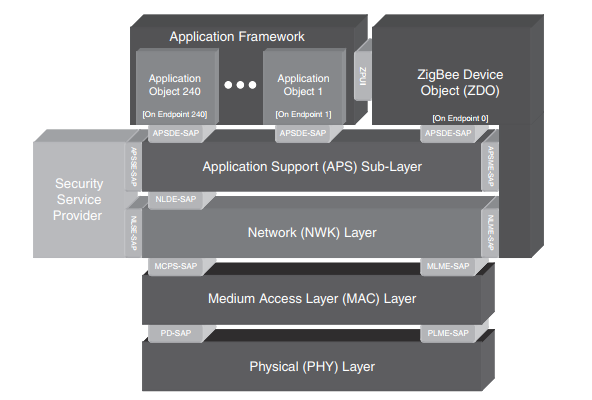
\includegraphics[scale=0.5]{camadaszigbee} 
		\caption*{Fonte: \cite{gislason2008zigbee}.}
		\label{fig:camadaszigbee}
\end{figure} 

Quanto a topologia de rede, o ZigBee opera em topologias de estrela, malha e árvore. Entretanto, independente de topologia, o ZigBee atua sobre uma \textit{Personal Area Network} (ou PAN) criada em um \textit{identifier} (ID) específico, esta PAN possui os nós (módulos físicos do ZigBee) onde cada nó da topologia pode ser um dos três tipos de nós do protocolo, sendo eles o coordenador, o roteador e o \textit{end-point} \cite{elahi2009zigbee}. O coordenador tem a responsabilidade de criar a rede PAN, o roteador repassa pacotes enviados de \textit{end-points} e os ditos \textit{end-points} são os nós que possuem os sensores e atuadores da rede, uma característica específica deste tipo de nós é que os mesmos podem entrar em \textit{stand-by} para consumir menos energia quando não estão operando.    

\subsection{Estrutura de envio}
O ZigBee possui uma estrutura definida para o envio de dados sem fio. O quadro de dados do protocolo possui alguns \textit{stamps} para envio dos dados de forma que o destino das mensagens possa ser definido no envio, possua um indicador de força do sinal com o byte chamado de RSSI (\textit{Received Signal Strength Indicator}) e possibilita o envio de mensagens de sucesso de transmissão. 

A Figura \ref{fig:xbeeframe} exibe alguns quadros que podem ser enviados nos módulos XBee, da empresa \textit{Digi International}. É possível observar na estrutura dos quadros alguns \textit{stamps} obrigatório que permitem que as características citadas sejam possíveis. O primeiro byte é o delimitador de início do quadro, ele indica que a partir daquele byte existe um quadro válido, os dois próximos bytes são referentes ao início das informações do quadro (\textit{Most Significant Byte}) e ao fim das informações (\textit{Least Significant Byte}. Os próximos \textit{N} bytes são referentes aos dados do quadro, que variam de acordo com o tipo de quadro enviado, contudo, esta parte inicia com um byte de identificação e prossegue com seus \textit{N} bytes de dados. Por fim é enviado um byte de \textit{checksum}, este byte é utilizado para verificar a integridade dos componentes\cite{xbeetutorial}.       

\begin{figure}[!htb]
	\centering
		\caption{Alguns quadros de envio dos modelos XBee.}
		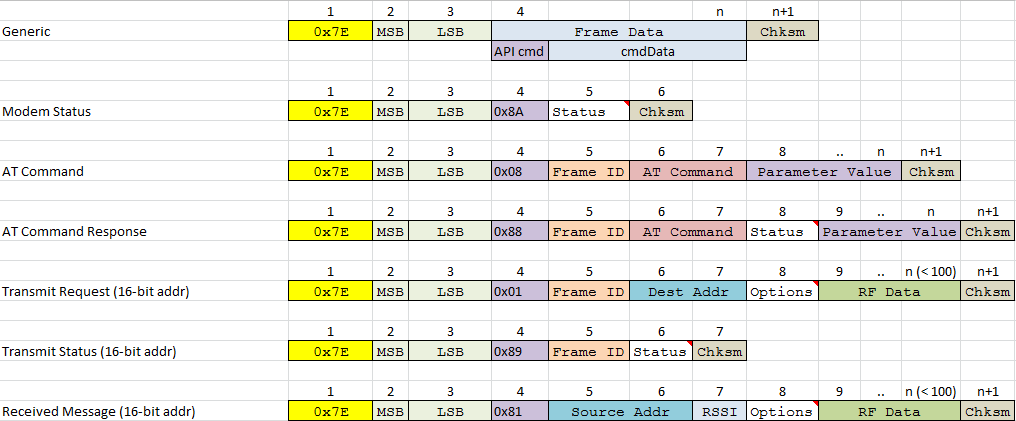
\includegraphics[scale=0.5]{xbeeframe} 
		\caption*{Fonte: \cite{xbeetutorial}.}
		\label{fig:xbeeframe}
\end{figure} 


\section{Software}
\label{sec:software}

O \textit{software} é parte essencial deste trabalho. Todas as grandezas adquiridas pelos sensores apresentados na seção \ref{sec:sensores} e concentrados nos microcontroladores revisados na seção \ref{sec:microcontroladores} devem ser submetidas a um \textit{software} para transformação destes dados em informações. As seções a seguir revisam qual tarefa cada sub sistema deve realizar para alcançar os objetivos propostos na seção \ref{sec:objetivos}.  

\subsection{Aquisição de dados}
\label{sec:aquisicaodedados}

O \textit{software} de aquisição de dados é a primeira interação dos dados vindos dos sensores com algum tipo de tratamento. Este subsistema não é o foco deste trabalho, porém ele deve ser revisado pois caso o \textit{software} principal traga alguma mudança substancial na forma de tratamento dos dados, os subsistemas de aquisição dentro dos microcontroladores deve ser atualizado para satisfazer quaisquer novos requisitos.

Este subsistema é produzido por três motivos: ele deve realizar a comunicação entre múltiplos microcontroladores em caso de uso de arquitetura distribuída, realizar qualquer cálculo inicial para demonstração de informações no painel e ele deve preparar os dados para passagem para o subsistema de tratamento de dados \cite{racecarInstrumentationFor2012}\cite{projetoMiniBaja2006}\cite{designAndImplementation2015}\cite{Dias2010}\cite{Nunes2016}. A Figura \ref{fig:aquisicaodiagrama} demonstra como este subsistema funciona, os sensores capturam as grandezas desejadas e enviam os dados para o SCOB via chicote elétrico. As saídas dos sensores são conectadas nas entradas digitais ou analógicas do microcontrolador. O \textit{software} atual é feito em C e utiliza a biblioteca padrão do Arduino, visto o uso do Arduino Nano V3. Os dados são armazenados em variáveis e a cada ciclo do programa, os mesmos são enviados via ZigBee.      

\begin{figure}[!htb]
	\centering
		\caption{Diagrama exemplificando funcionamento do sistema de aquisição.}
		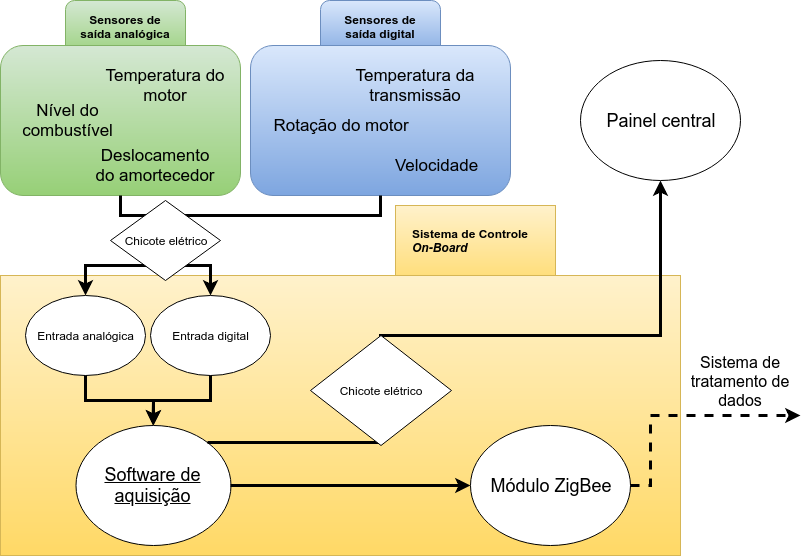
\includegraphics[scale=0.5]{aquisicaodiagrama} 
		\caption*{Fonte: Autor.}
		\label{fig:aquisicaodiagrama}
\end{figure} 


\subsection{Tratamento de dados}

O sistema de tratamento de dados deve receber as informações fornecidas pelo meio de transporte de informação, neste caso o módulo ZigBee, e com esses dados atualizar o ambiente e informar a equipe dos boxes dos dados mais importantes sobre o veículo. Este sistema pode ser feito para dados recebidos posteriormente a testes ou com telemetria, sendo feita análises em tempo real. Algumas análises de dados que podem ser realizadas neste \textit{software} seriam torção do chassi, temperatura do motor em relação a velocidade do veículo, tempo de prova, entre outras informações. 

As equipes de automobilismo não divulgam muitas informações sobre seus sistemas de tratamento de dados. A exceção é quando estes sistemas utilizam de plataformas de empresas privadas para codificação destes \textit{software}, nestes casos os artigos comentam que estas plataformas são utilizadas para criação da GUI (Graphical User Interface) e geralmente usadas em conjunto com dispositivos de aquisição de dados também adquiridos de empresas privadas \cite{applicationOfData2010}\cite{vehicleDataAcquisition2014}\cite{designAndImplementation2015}\cite{developmentOfAn2016}. Contudo estas informações não são relevantes para o trabalho proposto na área de tratamento de dados, pois o sistema que deve ser desenvolvido para este fim deve ser projetado e executado junto a equipe Velociraptor com um requisito de baixo custo monetário. Um artigo revisado produziu sua própria plataforma de tratamento de dados em C e C++ \cite{racecarInstrumentationFor2012} e utiliza de alguns conceitos comentados na Seção \ref{sec:aquisicaodedados}, como utilização de \textit{comma-separated values} para formatação dos arquivos de dados. 

\begin{comment}

\subsection{Engenharia de software}
\label{sec:engenhariadesoftware}

A engenharia de \textit{software} é fundamentalmente o uso de processos para atingir uma meta com melhor qualidade, previsibilidade e economia. A engenharia de \textit{software} se baseia em princípios da engenharia para que suas atividades proposta, a fim de alcançar um objetivo final, sejam eles: interdependentes; com responsáveis (pessoas encarregadas de tarefas); e com entradas e saídas definidas \cite{wazlawick2013engenharia}. Os processos de engenharia de \textit{software} são feitos para o \textit{software} de forma genérica, sendo assim o cunho do projeto não deve ser um empecilho para a adoção das técnicas, processos e atividades. Em \citeonline{Pereira2012} é produzido um quadro com um conjunto de atributos que é desejável em qualquer sistema de \textit{software}. No Quadro \ref{fig:atributossoftware} é possível verificar os atributos relevantes para o trabalho proposto e alcançar-los é um objetivo específico deste trabalho, o que impulsiona o uso de alguns conceitos de tais processos.        


\begin{table}[!htb]
	\centering
		\caption{Tabela com atributos desejáveis em um \textit{software}.}
		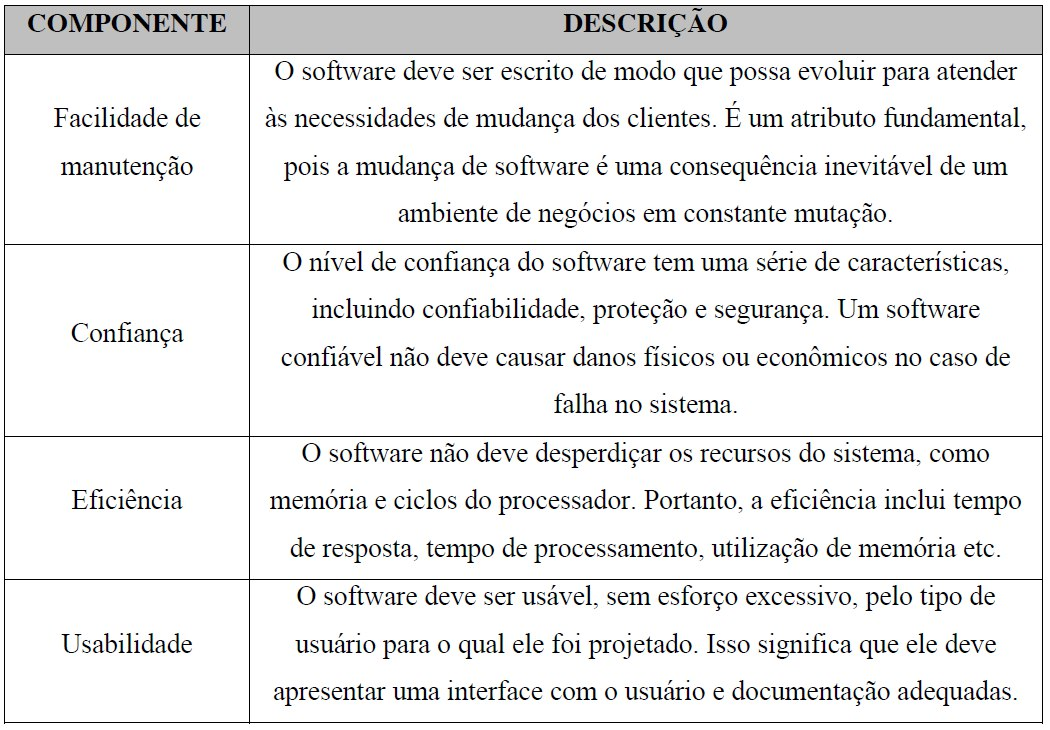
\includegraphics[scale=0.3]{atributossoftware} 
		\caption*{Fonte: \cite{Pereira2012}}
		\label{fig:atributossoftware}
\end{table} 

Existem dois tipos principais de abordagem quando se comenta em usar métodos de engenharia de \textit{software}, a primeira é a utilização de modelos de processos prescritivos. Os modelos prescritivos são aqueles que se baseiam em uma descrição, geralmente em requisitos levantados junto com o cliente, para criar processos a serem seguidos durante a execução do projeto \cite{wazlawick2013engenharia}. Alguns modelos que utilizam processos prescritivos são: o modelo cascata que introduz fases bem definidas e produção de documentação durante o processo; o modelo V que possui a execução de testes em diversos momentos em decorrer do projeto, o que enfatiza a importância dos mesmo para a construção do \textit{software}; o modelo espiral proposto por Boehm e com forte orientação a redução de riscos do projeto. 

O modelo evolucionário parece possuir maior relevância para o projeto proposto neste trabalho de conclusão de curso, nele o projeto é baseado em uma técnica de prototipagem conhecida como \textit{cornerstone}. Nesta técnica são construídos protótipos no decorrer do processo, para avaliar os aspectos do sistema e entender melhor os requisitos e reduzir riscos. A Figura \ref{fig:evolucionario} produzida por \citeonline{wazlawick2013engenharia} demostra um diagrama de atividades UML simplificado para um prototipo genérico utilizando o modelo de prototipagem evolucionária. Uma desvantagem citada no texto é em relação a dificuldade de gerência do projeto, pois é difícil manter uma boa previsão de tempo para o mesmo devido a volatilidade das fases. Tal desvantagem pode ser superada com a ajuda de outro modelo sobre a prototipagem evolucionária, porém ao custo de aumento de complexidade.  


\begin{figure}[!htb]
	\centering
		\caption{Desenho exemplificando uma aplicação genérica do modelo evolucionário.}
		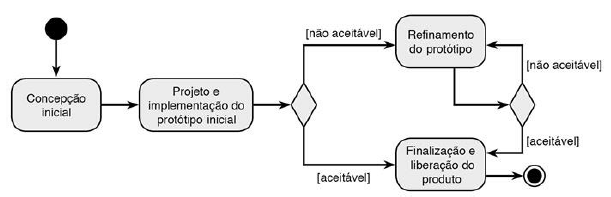
\includegraphics[scale=0.7]{evolucionario} 
		\caption*{Fonte: \cite{wazlawick2013engenharia}}
		\label{fig:evolucionario}
\end{figure} 

O outro tipo de abordagem para os métodos da engenharia de \textit{software} são os métodos ágeis. Criados para suprir a necessidade da indústria de lançar produtos com mudança constante de requisitos e imprescindibilidade de desenvolvimento rápido utilizando uma metodologia que melhora a produtividade geral dos seus usuários. Os métodos ágeis se apoiam em uma atitude de incremento sobre mudanças, sejam elas de requisitos, desenvolvimento ou entrega \cite{Sommerville2010}. Contudo a melhor forma de explicar a filosofia do método ágil é com o manifesto para desenvolvimento ágil de \textit{software} \cite{manifestoagil}, este comenta que os indivíduos e interações devem estar acima dos processos e ferramentas, \textit{software} em funcionamento sobre documentação abrangente, colaboração com o cliente e resposta constante a mudanças. 

Existem vários modelos de métodos ágeis e o escolhido para ser focado neste trabalho foi o método \textit{SCRUM}. Esta escolha foi feita devido ao foco em produtividade do método e experiência prévia do autor no uso do mesmo. 

\subsubsection{SCRUM}
\label{sec:scrum}

O \textit{SCRUM} é um método que foca em trazer o cliente para perto da equipe de desenvolvimento e com isto fazer entregas assertivas em ciclos mensais ou semanais, dependendo do tamanho da equipe de desenvolvimento. Existem três perfis importantes no método, eles são os seguintes \cite{scrum}\cite{wazlawick2013engenharia}:

\begin{itemize}
	\item \textbf{SCRUM master:} É um facilitador na tomada de decisão em relação as mecânicas do \textit{SCRUM};
	\item \textbf{Product owner:} O interessado no produto, quem irá utilizar os resultados, este papel tem maior peso na decisão de tarefas a serem feitas; e
	\item \textbf{SCRUM team:} Esta é a equipe de desenvolvimento, entre 6 a 10 pessoas.
\end{itemize} 

O método trabalha em ciclos de desenvolvimento de semanas ou até mesmo um mês. Em cada ciclo, tarefas são levantadas da necessidade do cliente e colocadas no \textit{sprint} da equipe. As tarefas ficam em um \textit{product backlog} e são avaliadas em todo início de ciclo, se forem aprovadas elas são adicionadas ao \textit{sprint backlog} e trabalhadas durante o ciclo. A Figura \ref{fig:scrumquadro} trás um exemplo de um quadro genérico de \textit{SCRUM} produzido por \citeonline{wazlawick2013engenharia}. Os quadros de \textit{SCRUM} e algumas outras mecânicas do modelo podem ser alterados para se encaixar melhor com o cenário em que elas são empregadas \cite{Sommerville2010}, na Seção \ref{sec:objetivos} é proposto uma utilização de um quadro específico para o cenário do trabalho. 


\begin{figure}[!htb]
	\centering
		\caption{Exemplo de um quadro genérico de \textit{SCRUM}.}
		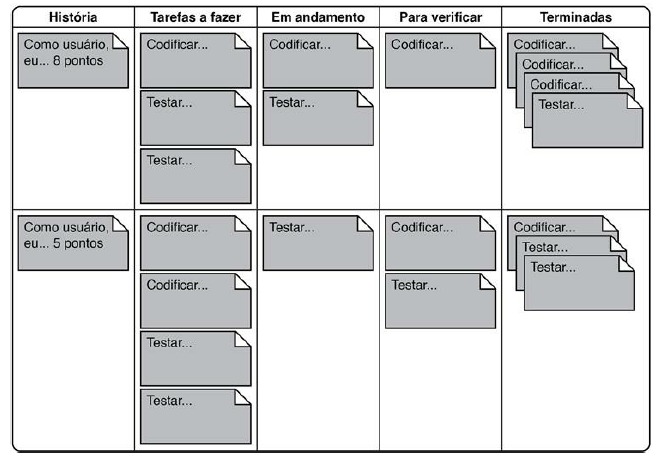
\includegraphics[scale=0.7]{scrumquadro} 
		\caption*{Fonte: \cite{wazlawick2013engenharia}}
		\label{fig:scrumquadro}
\end{figure} 


\end{comment}

